%%% Jim Ashe (jim.ashe@wgu.edu; x4209)%%%%
\documentclass{exam}
\usepackage{WGU_worksheet_preamble}

%%%%%%%%%%%%%%%%%%%%%%%%%%%%%%%%%%%%%%%%%%
%%header%%%%%%%%%%%%%%%%%%%%%%%%%%%%%%%%%%
\headrule
\header{ \href{mailto:jim.ashe@wgu.edu?subject=C960: probability worksheet}{Dr.\,Jim Ashe } \\ \textbf{C960: Discrete Probability}}
{Practice Problems}
{\href{https://www02.timetrade.com/app/wgu-mentoring/workflows/WGU200/schedule?wfsid=16a5bb8c-baba97f6-16a5bc0d-baba97f6-00000003-s0k1arrrqdocp902m3b135gfjgbbqcag&locationId=course_mentoring&appointmentTypeGroupId=C960&resourceId=any}{
\includegraphics[scale=.65]{timetradeMC.png}}}
%%%%%%%%%%%%%%%%%%%%%%%%%%%%%%%%%%%%%%%%%
\lfoot{}
\cfoot[]{Page \thepage\ of \numpages}
\rfoot{\today}
%%%%%%%%%%%%%%%%%%%%%%%%%%%%%%%%%%%%%%%%%
%\printanswers
%%%set box settings%%%%
% \newmdenv[innerlinewidth=0.5pt, roundcorner=4pt,linecolor=blueWGU,innerleftmargin=6pt, innerrightmargin=6pt,innertopmargin=6pt,innerbottommargin=6pt, backgroundcolor=lightBlueWGU!15!white]{myThm}


\begin{document}
            \small
\section*{\cChangey{-1.5} You \textbf{CANNOT} use this or any other formula sheet on the Assessment. You need to memorize this stuff }

\section*{Algorithms}
    \begin{multicols}{2}
        Here's a list of some functions listed from fast to slow:
        \begin{itemize}
            \item[] $\mathcal{O}(1)$ \textbf{Constant}
            \item[] $\mathcal{O}(\log(n))$ \textbf{Logarithmic}. 
            \begin{itemize}
                \item[] Ignore Log bases: $\log_{10}(n)=\log(n)$
                \item[] Same growth as $\log(n^{k})=k\log(n)$ 
            \end{itemize}
            
            \item[] $\mathcal{O}(\log^{c}(2n))$ \textbf{Polylogarithmic}
            \begin{itemize}
                \item[] Don't forget that: $\log^{c}x=(\log x)^{c}$.
            \end{itemize}
            \item[] $\mathcal{O}(n)$ \textbf{Linear}
            \item[] $\mathcal{O}(n\log(2n))$ \textbf{Linearithmic/Loglinear}
            \item[] $\mathcal{O}(n^{2})$ \textbf{Quadratic}
            \item[] $\mathcal{O}(n^{2}\log(2n))$
            \item[] $\mathcal{O}(n^{3})$ \textbf{Polynomial}
            \item[] $\mathcal{O}(2^{n})$ \textbf{Exponential} 
            \item[] $\mathcal{O}(n!)$
        \end{itemize}
        \columnbreak
        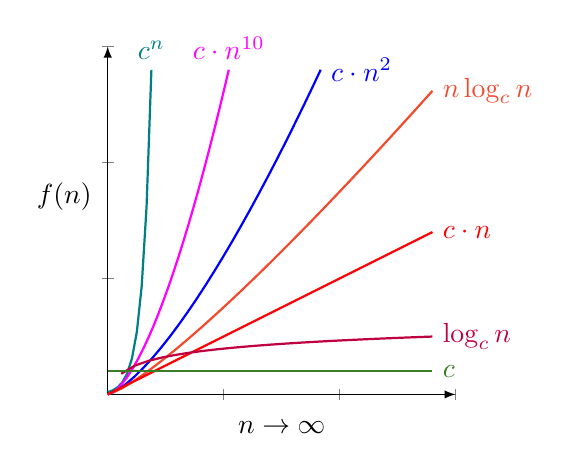
\begin{tikzpicture} 
            \begin{axis}[height=6cm, 
            	width=6cm,scale=1.0,
            	axis lines=middle,
            	xticklabels={,,}, yticklabels={,,},
            	axis line style={-latex}, 
            	xlabel={$n\rightarrow \infty$},
            	ylabel={$f(n)$},             	
            	x label style={at={(axis description cs:0.5,-0.05)},anchor=north},
            	y label style={at={(axis description cs:-0.125,.5)},anchor=south},
            	clip=false, %doesn't clip outside graph
            	%domain=0:100,
            	ymin=0,xmin=0,
            	ymax = 150,xmax=150
            	]
            	\addplot[teal, thick, samples=10, domain=0:18.835]{1.3^x} node[above]{$c^{n}$};
            	\addplot[Magenta, thick, domain=0:52.1936]{.25*x^1.6} node[above]{$c\cdot n^{10}$};
            	\addplot[blue, thick, domain=0:91.8315]{.25*x^1.4} node[right]{$c\cdot n^{2}$};
            	\addplot[RedOrange, thick, domain=0:140]{.13*(x+1)*ln(x+1)/ln(2)} node[right]{$n\log_{c}n$};
            	\addplot[red, thick, domain=0:140] {.5*x} node[right]{$c\cdot n$};
            	\addplot[purple, thick, domain=0:140]{3.5*ln(x)/ln(2)} node[right]{$\log_{c}n$};
            	\addplot[OliveGreen, thick, domain=0:140]{10} node[right]{$c$};
            \end{axis}
        \end{tikzpicture}
        \\ \textbf{Some properties} \\
            We ignore coefficients and log bases, but not exponent bases.
                \begin{itemize}
                    \item [\textbf{ex.}] $3\cdot5^{x}$ is $\mathcal{O}(5^{x})$
                \end{itemize}
        
            When adding functions, we only take the slowest function's Big-$\mathcal{O}$.
            \begin{itemize}
                \item[\textbf{ex.}] $0.01x^3+12x^{2}-2\log{37x}$ is $\mathcal{O}(n^{3})$
            \end{itemize}
            
            When multiplying functions, we take take the product of the functions' Big-$\mathcal{O}$. 
            \begin{itemize}
                \item[\textbf{ex.}] $x^{2}+2\in \mathcal{O}(n^{2})$ and $\log_{10}(x)\in \mathcal{O}(\log{n})$ so then \\
                $(x^{2}+2)(\log_{10}(x)) \text{is} \mathcal{O}(n^{2} \log(n))$
            \end{itemize}
    \end{multicols}

\section*{Advanced Counting}
\begin{multicols}{2}
    \begin{myThm}
        \textbf{Combination} Number ways to choose $k$ objects from a group of $n$ when \textit{order doesn't matter}:
        $${}_{n}C_{k}=\binom{n}{k}=\frac{n!}{n-r}!r!$$
    \end{myThm}
    
    \begin{myThm}
        \textbf{Permutation} Number ways to choose $k$ objects from a group of $n$ when \textit{order does matter}:
        $${}_{n}P_{k}=\frac{n!}{n-r}!$$
    \end{myThm}
\end{multicols}

\begin{myThm}
    \textbf{Binomial Theorem} 
    $$(a+b)^{n}=\sum^{n}_{k=0} \binom{n}{k} a^{k}b^{n-k}$$
    This gives us the following identity:
    $$\binom{n}{0}-\binom{n}{1}+\binom{n}{2}-\cdots (-1)^{n}\binom{n}{n}=0$$
\end{myThm}
\vspace{10pt}

\section*{Discrete Probability}  
    \begin{itemize}
        \item $P(A)$ is the probability of event $A$ happening.
        \item $P(\overline{A})=1-P(A)$ is the probability of event $A$ \textbf{not }happening. 
        \item $P(A|B)$ is the probability of event $A$ \textit{given} that $B$ has already happened. When $A$ and $B$ are independent, $P(A|B)=A$.
        \item $P(A\cap B)=P(A|B)P(B)$ is the probability of event $A$ \textit{and} $B$ happening.  
        \item $P(A\cup B)=P(A)+P(B)-P(A\cap B)$ is the probability of the $A$ \textit{or} $B$ happening.
    \end{itemize}
\begin{myThm}
\textbf{Bayes' Theorem:} For events $X$ and $F$ from a common sample space where $P(X),P(F)\neq 0$, 
    \begin{equation}\label{eqn: bayes1}
        P(F|X)=\frac{P(X|F)P(F)}{P(X)}\tag{version 1}
    \end{equation}

    and equivalently,
    \begin{equation}\label{eqn: bayes2}
        P(F|X)=\displaystyle \frac{P(X|F)P(F)}{P(X|F)P(F)+P(X|\overline{F})P(\overline{F})}\tag{version 2}
    \end{equation}
    While the first version does not appear in our textbook or pre-assessment practice problems, this equivalent definition is listed in the lesson summary. 
    
    Note that $P(F\cap X)=P(X|F)P(F)$. So version 1 is often shown as:
    \begin{equation}\label{eqn: bayes3}
        P(F|X)=\frac{P(X\cap F)}{P(X)}\tag{version 3}
    \end{equation}
\end{myThm}
\vspace{10pt}

\begin{myThm}
    \textbf{Expected Value} The \emph{expected value} of a discrete random variable $X$ is $$E[X]=\sum_{s\in S}X(s)p(s)$$ where $S$ is the set of possible outcomes of $X$, $p(s)$ is the probability of outcome $s$, and $X(s)$ is the value of $X$ for $s$.
\end{myThm}

\section*{Number Theory}

Stuff to add?
\begin{itemize}
    \item modular arithmetic basics
    \item needed modular arithmetic properties
    \item Euclidean algorithm
    \item Extended Euclidean Algorithm
    \item Encryption 
\end{itemize}

\section*{Recursion and Induction}
Stuff to add?
\begin{itemize}
    \item Label for Induction parts
    \item Summation formulation label? 
\end{itemize}

\end{document}
